\documentclass[tikz]{standalone}
\usetikzlibrary{shapes.geometric}
\begin{document}%
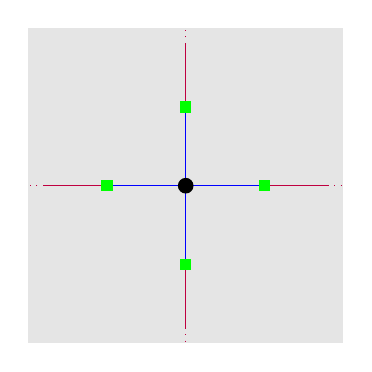
\begin{tikzpicture}
\fill[gray!20] (-2,-2) rectangle (2,2);

\coordinate (A) at (0,0);

\coordinate (B0) at (1,0);
\coordinate (B1) at (0,1);
\coordinate (B2) at (-1,0);
\coordinate (B3) at (0,-1);

\draw[blue] (A) -- (B0);
\draw[blue] (A) -- (B1);
\draw[blue] (A) -- (B2);
\draw[blue] (A) -- (B3);

\draw[purple] (B0) -- (1.8,0);
\draw[purple,dotted] (1.8,0) -- (2,0);
\draw[purple] (B1) -- (0,1.8);
\draw[purple,dotted] (0,1.8) -- (0,2);
\draw[purple] (B2) -- (-1.8,0);
\draw[purple,dotted] (-1.8,0) -- (-2,0);
\draw[purple] (B3) -- (0,-1.8);
\draw[purple,dotted] (0,-1.8) -- (0,-2);

\node[circle,fill=black,inner sep=2pt] at (A) {};

\foreach \x in {0,1,...,3}
\node[rectangle,fill=green,inner sep=2pt] at (B\x) {};

\end{tikzpicture}%
\end{document}
